% backpatch-chain.tex

% !TEX program = pdflatex
\documentclass[tikz]{standalone}
\usetikzlibrary{shapes.multipart, positioning}

\newcommand{\red}[1]{\textcolor{red}{#1}}
\newcommand{\blue}[1]{\textcolor{blue}{#1}}
\newcommand{\teal}[1]{\textcolor{teal}{#1}}
\newcommand{\purple}[1]{\textcolor{purple}{#1}}
\newcommand{\falselist}{\mathit{falselist}}
\newcommand{\truelist}{\mathit{truelist}}
\newcommand{\nextlist}{\mathit{nextlist}}

\newcommand{\cgets}{\red{\;\gets\;}}
\newcommand{\cto}{\blue{\;\to\;}}

\begin{document}
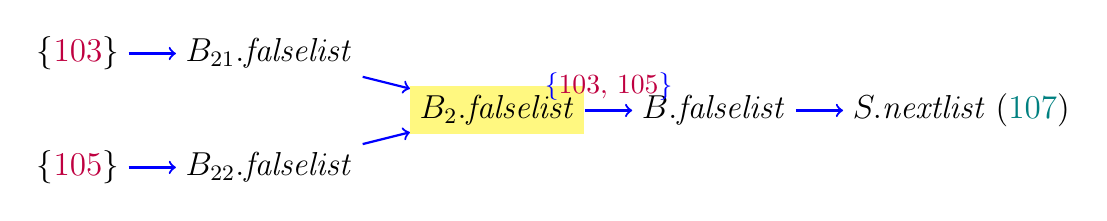
\begin{tikzpicture}[node distance = 0.1cm and 0.6cm,
    pass/.style = {->, blue, thick},
    list/.style = {font = \large}]
  \node (E) [list, rectangle, fill = yellow!50] {$B_{2}.\falselist$};
  \node (F) [right = of E, list] {$B.\falselist$};
  \node (G) [right = of F, list] {$S.\nextlist \;(\teal{107})$};

  \node (B) [above left = of E, list] {$B_{21}.\falselist$};
  \node (A) [left = of B, list] {\{\purple{103}\}};

  \node (D) [below left = of E, list] {$B_{22}.\falselist$};
  \node (C) [left = of D, list] {\{\purple{105}\}};

  \draw[pass] (A) -- (B);
  \draw[pass] (C) -- (D);
  \draw[pass] (B) -- (E);
  \draw[pass] (D) -- (E);
  \draw[pass] (E) to node[above]{\{\purple{103, 105}\}} (F);
  \draw[pass] (F) -- (G);
\end{tikzpicture}
\end{document}